\chapter{Data presentation and analysis}
\label{chap:dataanalysis}

The prove of principle type of review was carried out on 8 from 10 planed participants. The number of participants was decreased because all information that was needed for further evaluation was already gather at this point and more test persons would not provide any new relevant data. Furthermore, the usability experiment focused more on gathering qualitative data than on quantitative data collection. Additionally, the youngest participant was three years old which deviates from the planed minimum age of two years. During the test sessions it turned out that the four and three years old participants already struggled to carry out the task which led to the conclusion that a toddler of two years of age would not have the expected understanding and motor development. The age and gender distribution of the prove of principle type of review is presented visually in table \ref{tab:participanttable}. Each participant was right handed and had no previous experience with hand-free gesture based games.


%all were right handed and novice users

\renewcommand{\arraystretch}{1.5}
 \begin{table}[h]
     \centering
     \begin{tabular}{c|c|c|c|c|c|c|c}
     \hline
        \multicolumn{1}{|l|}{\textbf{AGE:}}  &
        \multicolumn{1}{l|}{3}  &     
        \multicolumn{1}{l|}{4}  & 
        \multicolumn{1}{l|}{5}  & 
        \multicolumn{1}{l|}{7}  & 
        \multicolumn{1}{l|}{8}  & 
        \multicolumn{1}{l|}{9}  & 
        \multicolumn{1}{l|}{13} \\ \hline
        \multicolumn{1}{|l|}{\textbf{AMOUNT:}} &
        \multicolumn{1}{l|}{1}  &
        \multicolumn{1}{l|}{1}  &
        \multicolumn{1}{l|}{1}  &
        \multicolumn{1}{l|}{2}  &
        \multicolumn{1}{l|}{1}  &
        \multicolumn{1}{l|}{1}  &
        \multicolumn{1}{l|}{1}  \\ \hline
        \multicolumn{1}{|l|}{\textbf{GENDER:}}  &
        \multicolumn{1}{|l|}{F} &
        \multicolumn{1}{l|}{M}  &
        \multicolumn{1}{l|}{M}  &
        \multicolumn{1}{l|}{F/M}&
        \multicolumn{1}{l|}{F}  &
        \multicolumn{1}{l|}{M}  &
        \multicolumn{1}{l|}{F}  \\ \hline
        \multicolumn{1}{|l|}{\textbf{L/R HANDED:}} &
        \multicolumn{1}{|l|}{R} &
        \multicolumn{1}{l|}{R}  &
        \multicolumn{1}{l|}{R}  &
        \multicolumn{1}{l|}{R}  &
        \multicolumn{1}{l|}{R}  &
        \multicolumn{1}{l|}{R}  &
        \multicolumn{1}{l|}{R}  \\ \hline
        \multicolumn{1}{|l|}{\textbf{NOVICE/EXPERT:}} &
        \multicolumn{1}{|l|}{N} &
        \multicolumn{1}{l|}{N}  &
        \multicolumn{1}{l|}{N}  &
        \multicolumn{1}{l|}{N}  &
        \multicolumn{1}{l|}{N}  &
        \multicolumn{1}{l|}{N}  &
        \multicolumn{1}{l|}{N}  \\ \hline
     \end{tabular}
     \caption{Presentation of participants}
     \label{tab:participanttable}
 \end{table}
 

The age of the participant ranged from three to 13 years and included a mixture of boys and girls. 50\texttt{\%} boys and 50\texttt{\%} girls was a good balanced gender distribution. An equal distribution of gender is crucial when doing scientific research, since both genders have its own distinct characteristics. Regarding the age distribution, table  \ref{tab:agestatistic} presents a statistical calculation for age distribution in this study.
Additionally, figure \ref{fig:finishedgame} shows that 87,5 \texttt{\%} did actually finished the game at the first attempt. This illustrates that the game was challenging but not impossible. 

 %A graphical presentation of age and gender distribution is illustrated in figure \ref{fig:agedistribution} and figure \ref{fig:genderdistribution}. 


\renewcommand{\arraystretch}{1.5}

\begin{table}[!ht]
    \centering
    \begin{tabular}{c|c|c|c}
    \hline
        \multicolumn{1}{|c|}{MEAN} &
        \multicolumn{1}{c|}{MEDIAN} &
        \multicolumn{1}{c|}{MODE} &
        \multicolumn{1}{c|}{STANDARD DEVIATION}\\ \hline
       \multicolumn{1}{|c|}{7} &
        \multicolumn{1}{c|}{7} &
        \multicolumn{1}{c|}{7} &
        \multicolumn{1}{c|}{2,96} \\ \hline
    \end{tabular}
    \caption{Average age of participants}
    \label{tab:agestatistic}
\end{table}



%\begin{figure}[!ht]
%    \centering
%    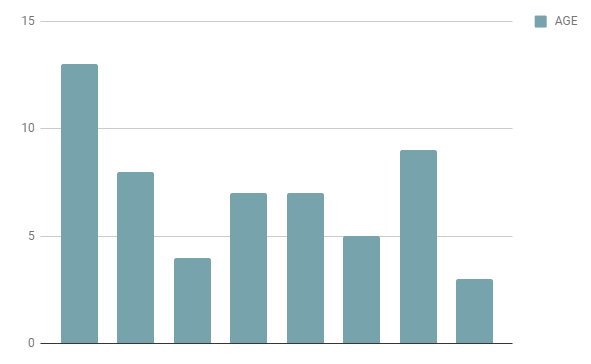
\includegraphics[width=.6\textwidth]{figures/agedistribution.png}
%    \caption{Diagram: Age distribution}
%    \label{fig:agedistribution}
%\end{figure}
%\begin{figure}[!ht]
%    \centering
%    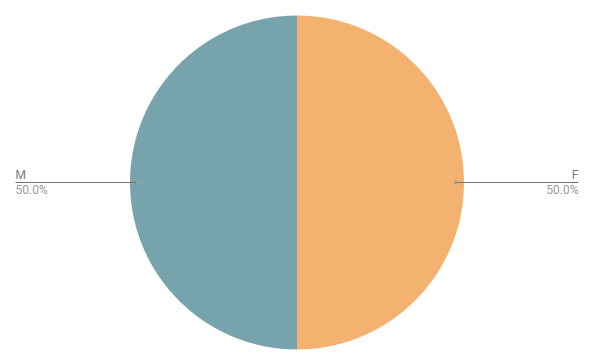
\includegraphics[width=.4\textwidth]{figures/genderdistribution.png}
%    \caption{Percentage of gender distribution}
%    \label{fig:genderdistribution}
%\end{figure}
\begin{figure}[!ht]
   \centering
    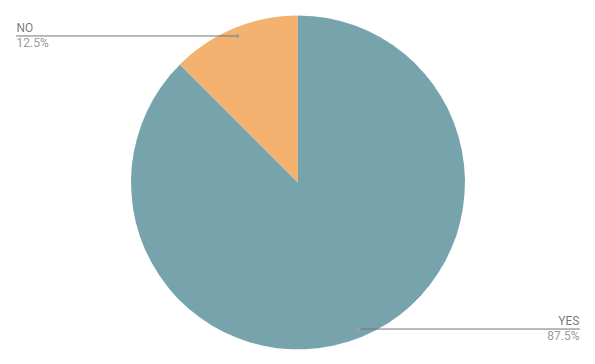
\includegraphics[width=.4\textwidth]{figures/finishedgame.png}
    \caption{Percentage of children who finished the game}
    \label{fig:finishedgame}
\end{figure}

\newpage


\section{Data extracted from the experiment and questionnaire}
The primary parameters in this experiment are \textit{time} and \textit{hits} where time is in relation to hits. The less time needed to finished the game and the less amount of hits counted during the game the better.
The closed-end questionnaire were original scale either with good-ok-bad or easy-ok-hard. This scale was transformed in numbers where good/easy represents number 1, ok represents number 2 and bad/hard represents number 3.
Sometimes, a participant did not want to answer the question (NA) or did not know (NK) the answer of a question. Since this study is based on voluntary and all compulsion could bias the outcome, the children were never force to respond to a question if they did not want to.

\subsection{Result of age group 1}
In this group, the age of the children ranged from three to five years. Most significant for this group is the less developed motor skills. Hand and finger size is substantial factor as well. 
The charts in figure \ref{fig:agegroup1} illustrate the outcome of the usability test. Participant \texttt{\# 6} did complete all three rounds and had the best time / hits score. He also showed that he had the best understanding of the concept in this group.
Table \ref{tab:closedendedquestiongroup1} presents the scoring for closed-ended follow up questions. It illustrates the difficulty of interacting and navigating touch-less. Although, the exercise was challenging for this group, they still liked the game.
Due to the age aspect, they could not respond to some of the open-end questions. However, the mole figure was pointed out as the best liked part of the game.
To conclude, touch-less gesture based interactions do need certain motor skills and spatial understanding of the concept. Unfortunately, the experiment showed that this is not ensured in children younger than 4.   


\begin{figure}[!ht]

    \centering
    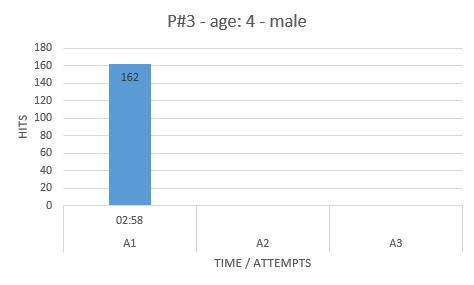
\includegraphics[width=.6\textwidth]{figures/p3.png}
   %  \caption{Participant \texttt{\#}3}
    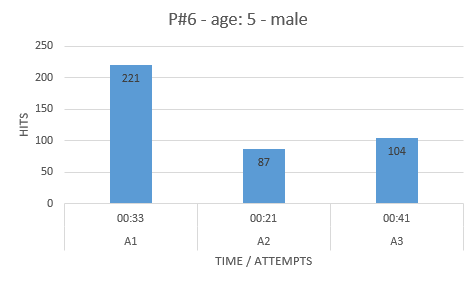
\includegraphics[width=.6\textwidth]{figures/p6.png}
 %   \caption{Participant \texttt{\#}6}
        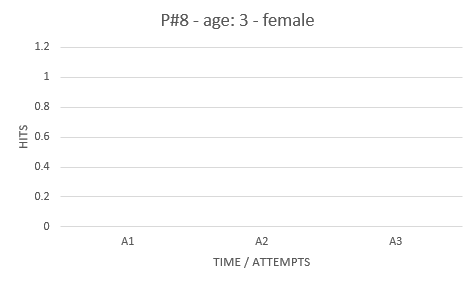
\includegraphics[width=.6\textwidth]{figures/p8.png}
    \caption{Time/hit parameters. Data presentation of age group 1. Participants \texttt{\#}3, 6 and 8}
    \label{fig:agegroup1}
\end{figure}

\begin{table}[!ht]
    \centering
    \begin{tabular}{c|c|c|c|c}
    \hline
    \multicolumn{1}{|c|}{\textbf{Question/participant}} &
    \multicolumn{1}{c|}{\textbf{Q1}} &
    \multicolumn{1}{c|}{\textbf{Q3}} &
    \multicolumn{1}{c|}{\textbf{Q4}} &
    \multicolumn{1}{c|}{\textbf{Q5}} \\ \hline
    \multicolumn{1}{|c|}{\textbf{P\texttt{\#}3}} &
    \multicolumn{1}{c|}{3} &
    \multicolumn{1}{c|}{3} &
    \multicolumn{1}{c|}{3} &
    \multicolumn{1}{c|}{1} \\ \hline
    \multicolumn{1}{|c|}{\textbf{P\texttt{\#}6}} &
    \multicolumn{1}{c|}{3} &
    \multicolumn{1}{c|}{3} &
    \multicolumn{1}{c|}{1} &
    \multicolumn{1}{c|}{1} \\ \hline
    \multicolumn{1}{|c|}{\textbf{P\texttt{\#}8}} &
    \multicolumn{1}{c|}{-} &
    \multicolumn{1}{c|}{-} &
    \multicolumn{1}{c|}{-} &
    \multicolumn{1}{c|}{-} \\ \hline
    \end{tabular}
    \caption{Closed-ended questions - group 1}
    \label{tab:closedendedquestiongroup1}
\end{table}

\begin{table}[!ht]
    \centering
    \begin{tabular}{c|c|c|c|c}
    \hline
  %  \rowcolor{1}{green}
    \multicolumn{1}{|c|}{\textbf{Question/participant}} &
    \multicolumn{1}{c|}{\textbf{Q2}} &
    \multicolumn{1}{c|}{\textbf{Q6}} &
    \multicolumn{1}{c|}{\textbf{Q7}} &
    \multicolumn{1}{c|}{\textbf{Q8}} \\ \hline
    \multicolumn{1}{|c|}{\textbf{P\texttt{\#}3}} &
    \multicolumn{1}{c|}{NK} &
    \multicolumn{1}{c|}{mole} &
    \multicolumn{1}{c|}{NA} &
    \multicolumn{1}{c|}{NA} \\ \hline
    \multicolumn{1}{|c|}{\textbf{P\texttt{\#}6}} &
    \multicolumn{1}{c|}{NA} &
    \multicolumn{1}{c|}{mole} &
    \multicolumn{1}{c|}{navigate - pointer} &
    \multicolumn{1}{c|}{OK} \\ \hline
    \multicolumn{1}{|c|}{\textbf{P\texttt{\#}8}} &
    \multicolumn{1}{c|}{-} &
    \multicolumn{1}{c|}{-} &
    \multicolumn{1}{c|}{-} &
    \multicolumn{1}{c|}{-} \\ \hline
    \end{tabular}
    \caption{Open-ended questions - group 1}
    \label{tab:openendedquestiongroup1}
\end{table}

\newpage

\subsection{Result of age group 2}
Age group 2, concerned children from six to eight years of age. Their motor skills are more developed compare to age group 1 which again is reflected in the result of the usability test and questionnaire. All participants did finish the game and went through all three attempts (figure \ref{fig:agegroup2}). The test result varies from attempt to attempt and there is no significant structure which could lead to a clear assumption. Two of the participants had most hit-points at their last attempt which could be explained by inpatient behavior. On the other hand, one participant did very good at the last attempt. Again, this could be explained by a child's personality.
All participants in this group answered the closed-end question (table \ref{tab:closedendenquestiongroup2}) \textit{"safely"} and did not have any strong opinions regarding difficulty level or affinity for the game. However, the open-ended questions (table \ref{tab:openendedquestiongroup2}) revealed some more impressions. The biggest challenge for those children was to navigate the pointer and stay in the allowed area. Interestingly, one of the participant pointed out that not to touch the screen in order to control the game was problematic. 



\begin{figure}[!ht]
    \centering
    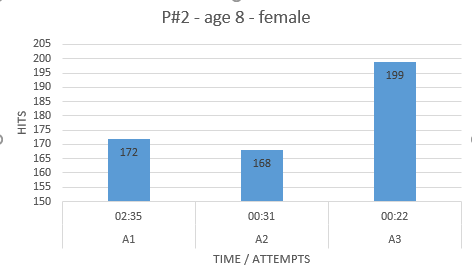
\includegraphics[width=.6\textwidth]{figures/p2.png}
    % \caption{Participant \texttt{\#}2}
    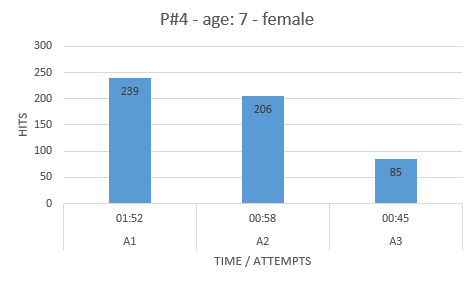
\includegraphics[width=.6\textwidth]{figures/p4.png}
   % \caption{Participant \texttt{\#}4}
        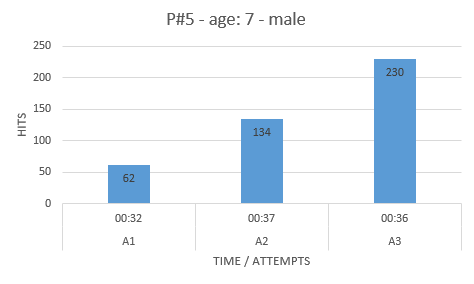
\includegraphics[width=.6\textwidth]{figures/p5.png}
    \caption{Time/hit parameters. Data presentation of age group 2. Participants \texttt{\#}2, 4 and 5}
    \label{fig:agegroup2}
\end{figure}

\begin{table}[!ht]
    \centering
    \begin{tabular}{c|c|c|c|c}
    \hline
    \multicolumn{1}{|c|}{\textbf{Question/participant}} &
    \multicolumn{1}{c|}{\textbf{Q1}} &
    \multicolumn{1}{c|}{\textbf{Q3}} &
    \multicolumn{1}{c|}{\textbf{Q4}} &
    \multicolumn{1}{c|}{\textbf{Q5}} \\ \hline
    \multicolumn{1}{|c|}{\textbf{P\texttt{\#}2}} &
    \multicolumn{1}{c|}{2} &
    \multicolumn{1}{c|}{2} &
    \multicolumn{1}{c|}{2} &
    \multicolumn{1}{c|}{1} \\ \hline
    \multicolumn{1}{|c|}{\textbf{P\texttt{\#}4}} &
    \multicolumn{1}{c|}{2} &
    \multicolumn{1}{c|}{2} &
    \multicolumn{1}{c|}{2} &
    \multicolumn{1}{c|}{2} \\ \hline
    \multicolumn{1}{|c|}{\textbf{P\texttt{\#}5}} &
    \multicolumn{1}{c|}{2} &
    \multicolumn{1}{c|}{2} &
    \multicolumn{1}{c|}{2} &
    \multicolumn{1}{c|}{2} \\ \hline
    \end{tabular}
    \caption{Closed-ended questions - group 2}
    \label{tab:closedendenquestiongroup2}
\end{table}

\begin{table}[!ht]
    \centering
    \begin{tabular}{c|c|c|c|c}
    \hline
    \multicolumn{1}{|c|}{\textbf{Question/participant}} &
    \multicolumn{1}{c|}{\textbf{Q2}} &
    \multicolumn{1}{c|}{\textbf{Q6}} &
    \multicolumn{1}{c|}{\textbf{Q7}} &
    \multicolumn{1}{c|}{\textbf{Q8}} \\ \hline
    \multicolumn{1}{|c|}{\textbf{P\texttt{\#}2}} &
    \multicolumn{1}{c|}{not to cross the line} &
    \multicolumn{1}{c|}{NA} &
    \multicolumn{1}{c|}{NA} &
    \multicolumn{1}{c|}{OK} \\ \hline
    \multicolumn{1}{|c|}{\textbf{P\texttt{\#}4}} &
    \multicolumn{1}{c|}{to move the pointer} &
    \multicolumn{1}{c|}{follow the white path} &
    \multicolumn{1}{c|}{navigate - pointer} &
    \multicolumn{1}{c|}{OK} \\ \hline
    \multicolumn{1}{|c|}{\textbf{P\texttt{\#}5}} &
    \multicolumn{1}{c|}{not to touch the screen} &
    \multicolumn{1}{c|}{NA} &
    \multicolumn{1}{c|}{NA} &
    \multicolumn{1}{c|}{OK} \\ \hline
    \end{tabular}
    \caption{Open-ended questions - group 2}
    \label{tab:openendedquestiongroup2}
\end{table}

\newpage

\subsection{Result of age group 3}
Group 3 was oldest group and had the most developed motor skills in this test row. However, one of the participants did not finished 3 attempts. It seemed that he got bored when he found out that the game just was a prototype and that he could cheat the system, something i also pointed out in the follow up questions and conversation.
Participants in this group thought that it was easy to hold up their hands during the game. None of them had strong opinions on the difficulty level of the task, they found it manageable.
Participant \texttt{\#}1 reported the same issue as participant \texttt{\#}5 namely, the unfamiliarity of touch-less navigation. 

\begin{figure}[!ht]
    \centering
    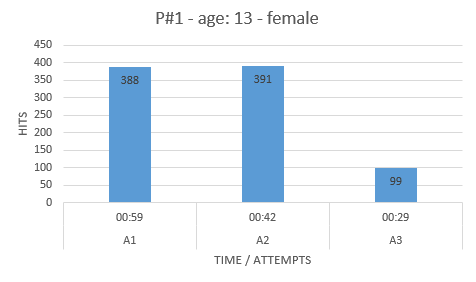
\includegraphics[width=.6\textwidth]{figures/p1.png}
     \caption{Participant \texttt{\#}1}
    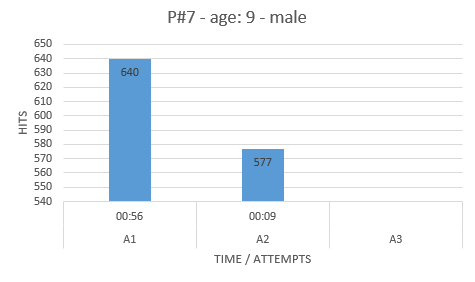
\includegraphics[width=.6\textwidth]{figures/p7.png}
    \caption{Time/hit parameters. Data presentation of age group 3. Participants \texttt{\#}1 and 7}

    \label{fig:agegroup3}
\end{figure}

\begin{table}[!ht]
    \centering
    \begin{tabular}{c|c|c|c|c}
    \hline
    \multicolumn{1}{|c|}{\textbf{Question/participant}} &
    \multicolumn{1}{c|}{\textbf{Q1}} &
    \multicolumn{1}{c|}{\textbf{Q3}} &
    \multicolumn{1}{c|}{\textbf{Q4}} &
    \multicolumn{1}{c|}{\textbf{Q5}} \\ \hline
    \multicolumn{1}{|c|}{\textbf{P\texttt{\#}1}} &
    \multicolumn{1}{c|}{2} &
    \multicolumn{1}{c|}{1} &
    \multicolumn{1}{c|}{2} &
    \multicolumn{1}{c|}{1} \\ \hline
    \multicolumn{1}{|c|}{\textbf{P\texttt{\#}7}} &
    \multicolumn{1}{c|}{2} &
    \multicolumn{1}{c|}{1} &
    \multicolumn{1}{c|}{1} &
    \multicolumn{1}{c|}{2} \\ \hline
    \end{tabular}
    \caption{Closed-ended questions - group 3}
    \label{tab:closedendedquestiongroup3}
\end{table}

\begin{table}[!ht]
    \centering
    \begin{tabular}{c|c|c|c|c}
    \hline
    \multicolumn{1}{|c|}{\textbf{Question/participant}} &
    \multicolumn{1}{c|}{\textbf{Q2}} &
    \multicolumn{1}{c|}{\textbf{Q6}} &
    \multicolumn{1}{c|}{\textbf{Q7}} &
    \multicolumn{1}{c|}{\textbf{Q8}} \\ \hline
    \multicolumn{1}{|c|}{\textbf{P\texttt{\#}1}} &
    \multicolumn{1}{c|}{not to touch the screen} &
    \multicolumn{1}{c|}{NA} &
    \multicolumn{1}{c|}{NA} &
    \multicolumn{1}{c|}{OK} \\ \hline
    \multicolumn{1}{|c|}{\textbf{P\texttt{\#}7}} &
    \multicolumn{1}{c|}{stay in tunnel} &
    \multicolumn{1}{c|}{challenging} &
    \multicolumn{1}{c|}{uncontrolled mole} &
    \multicolumn{1}{c|}{OK} \\ \hline
    \end{tabular}
    \caption{Open-ended questions - group 3}
    \label{tab:openendedquestiongroup3}
\end{table}


\subsection{Data analyzed as a whole}
By inspecting the data as a whole, a global relation between entity could so be demonstrated. For instance, investigating the relation between time and age group by using SPSS, a software for statistical analysis and data management, the data revealed that there is a connection between age and finishing time. Age group 3, containing a 13 year old and a nine year old participant, needed less time than age group 1, the youngest participant (age < 6). Consequently, the finish-time decreases by age which is an indication that the eye-hand coordination and fine motor performance are improving by increased age (Figure \ref{fig:relationTimeAge}).

\begin{figure}[!ht]
    \centering
    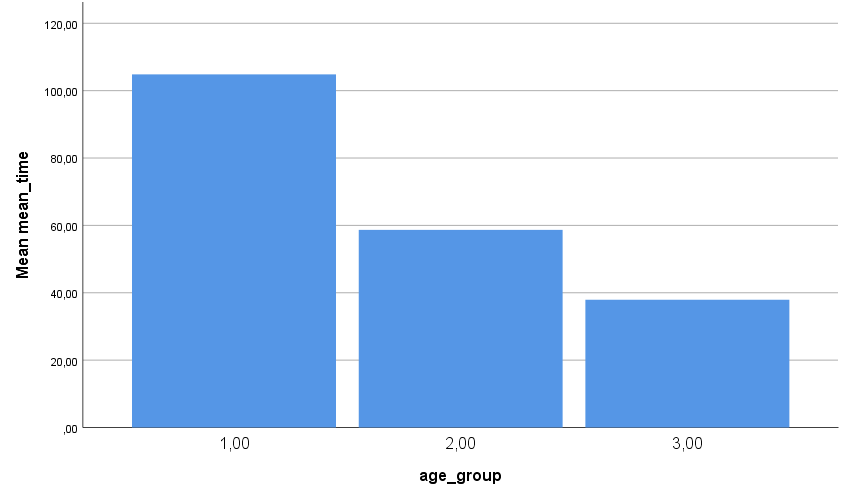
\includegraphics[width=.6\textwidth]{figures/relationTimeAge.png}
    \caption{Relation between age and time}
    \label{fig:relationTimeAge}
\end{figure}

Moreover, analyzing the follow up questions as a whole, revealed that age four and five found the task and the hand stabilization difficult. The older the participant were the more easier they found the task and the hand stabilization factor (figure \ref{fig:Q1}, \ref{fig:Q3}, \ref{fig:Q4}. Additionally, the graph in figure \ref{fig:Q5} illustrates that there is a great sympathy for the game by all participants.

\begin{figure}[!ht]
    \centering
    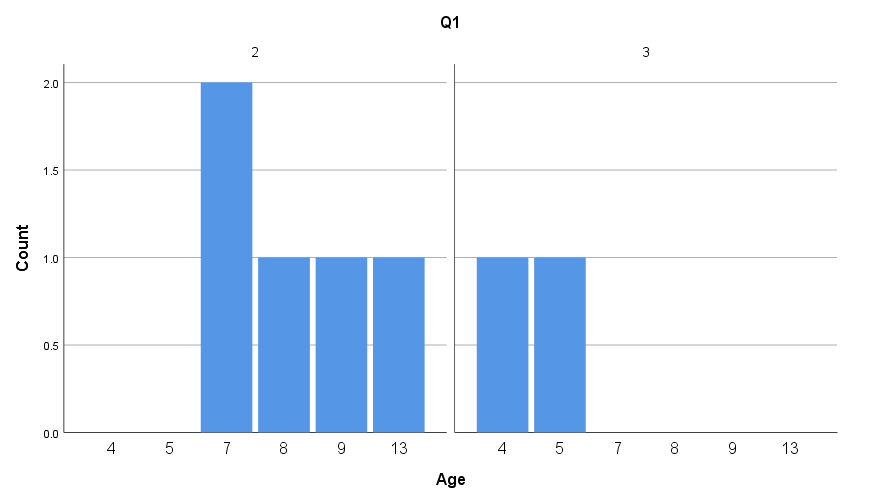
\includegraphics[width=.6\textwidth]{figures/Q1.png}
    \caption{Graphical presentation of question 1: Task difficulty}
    \label{fig:Q1}
\end{figure}
\begin{figure}[!ht]
    \centering
    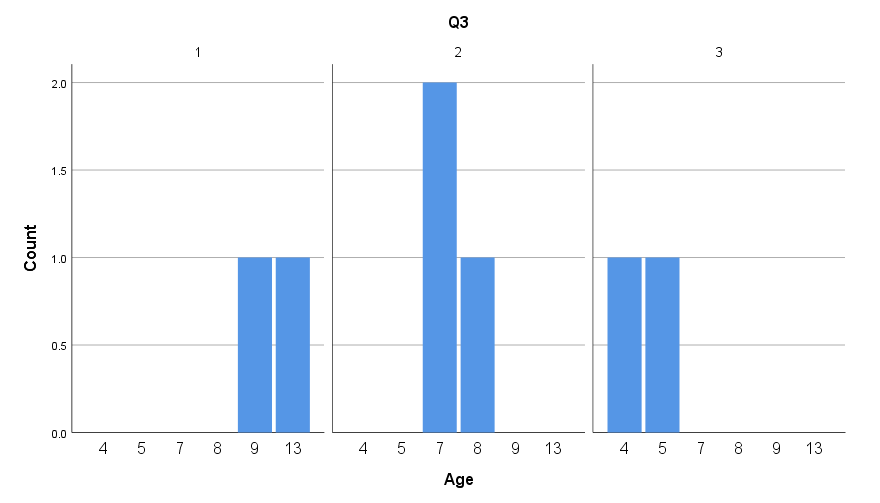
\includegraphics[width=.6\textwidth]{figures/Q3.png}
    \caption{Graphical presentation of question 3: Hand stabilization difficulty}
    \label{fig:Q3}
\end{figure}
\begin{figure}[!ht]
    \centering
    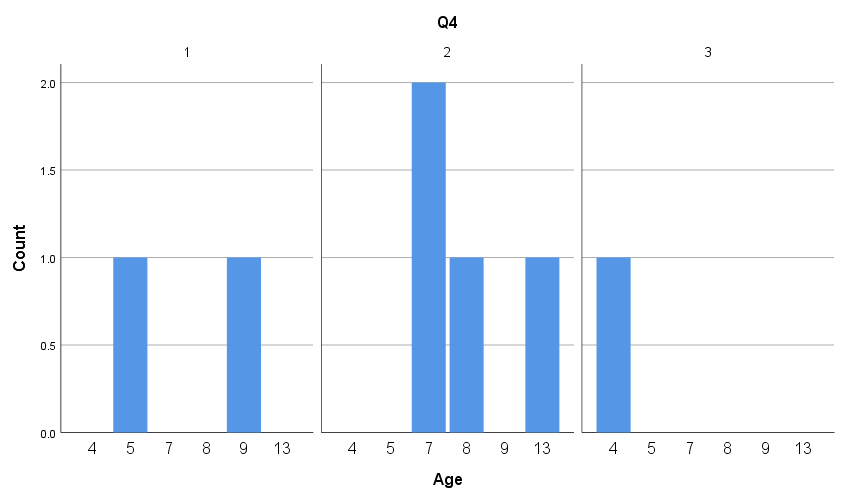
\includegraphics[width=.6\textwidth]{figures/Q4.png}
    \caption{Graphical presentation of question 4: Gesture and navigation difficulty}
    \label{fig:Q4}
\end{figure}
\begin{figure}[!ht]
    \centering
    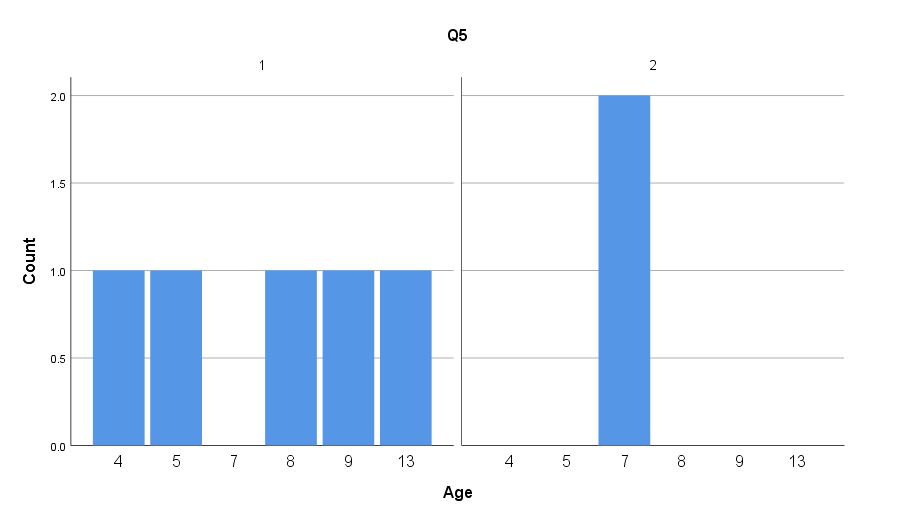
\includegraphics[width=.6\textwidth]{figures/Q5.png}
    \caption{Graphical presentation of question 5: Game sympathy }
    \label{fig:Q5}
\end{figure}



\section{Observation during the experiment}
During the experiment, the children were closely observed in order to gather information about how they handled the situation, expressed their feelings and coped with the game. Furthermore, some kids are not able to express themselves in words or get stressed when they have to replay a question. For that reason an observation could provide additional information.
There were observed several interesting issues relating to the touch-less concept. The youngest participants had too small fingers which gave them a big disadvantage when playing the game because the sensor did not recognized the stretched finger pose. They belonged to the group (\textit{group 1}) who at least understood the touch-less concept. They wanted to touched the screen in order to move the pointer or the mole. 
Most of the children were very curious about the Leap Motion sensor. They called it "the thing" because they never had seen something like that before. However, almost all of them were very eager to try the game. Especially the boys liked the idea of playing a touch-less game.
Unfortunately, not every child was patient enough. One participant was observed waving her hands and impatiently trying to make the pointer move to the mole. She also supported the pointing hand with her other hand, not because it was tiring to hold the hand above the device but rather as a help to navigate the finger in the right direction.  
Furthermore, the observation revealed that the most difficult gesture action during the sessions was the poking gesture. The game demanded a poking action in order to activate the walking mole.
Moreover, some users were very concentrated and focused on doing the task right. However they forgot about the right gesture, namely the poking finger. The finger needed to be completely stretched so the sensor could recognize the gesture. The consequence of the relaxed finger was that the system had trouble to distinguish the gesture.

Unfortunately, the prototype had some technical issues. The kids found out that it was possible to fool the system by directly going from start to finished without following the tunnel. Some other issues regarding time, hits and movement were observed as well. 

%finger too small
%touched the screen to navigate
%wave with finger because she didn't got it
%needed to support the pointing hand
%the poking part was most difficult 
%some were interest and ask what that thing is, 
%some were eager to to best
%the youngest did not understand the game and the concept
%bias:
%many took a shortcut "cheated"
%sometimes time stopped 
%sometimes the pointer did not react
%sometimes the pointer/mole jumped
%sometime the hit were not registered

%the deviation of time and hit was as expected varying. the study was not about reliaable paramenter but if it is possible to gather paramethers. since the game just was a prototype the result was expected not to be reliable
%mean:7 
%median: 7
%mode: 7
%standard deviation: 2,96
%Age from 3 - 13
%Gender 4 boys 4 girls
%13
%8
%4
%7
%7
%5
%9
%3

%Paramenters

%7 of 8 finished the game
%6 of 8 understood the game
% make a diagram to demonstrate
%https://blog.reachforce.com/blog/6-ways-to-make-your-data-analysis-more-reliable

